\section{Results}
\label{sec:result}
\subsection{Operator Code Complexity}
Lines of code in a software project is one indicator of system complexity. We
counted the lines of code (LOC) each Kubernetes operator codebase by the
language used. \figurename{ \ref{fig:loc}} shows that the total LOC follows a
power law distribution. The largest codebase, azure-service-operator, has 4.3
million LOC, while the smallest codebase, container-security-operator, has 7755
LOC. Most operators are written in Go while 3 are written in Java, and 1
written in Python. On average, 44.5\% of the total lines of code in the project
is the programming language that the operator is written in; 3

% \subsection{Operator Testing Code}
% Operators uses a variety of testing frameworks and tools for unit test,
% integration test, and end-to-end test.

% 90\% of operators have end-to-end tests

\begin{figure*}
    \centering
    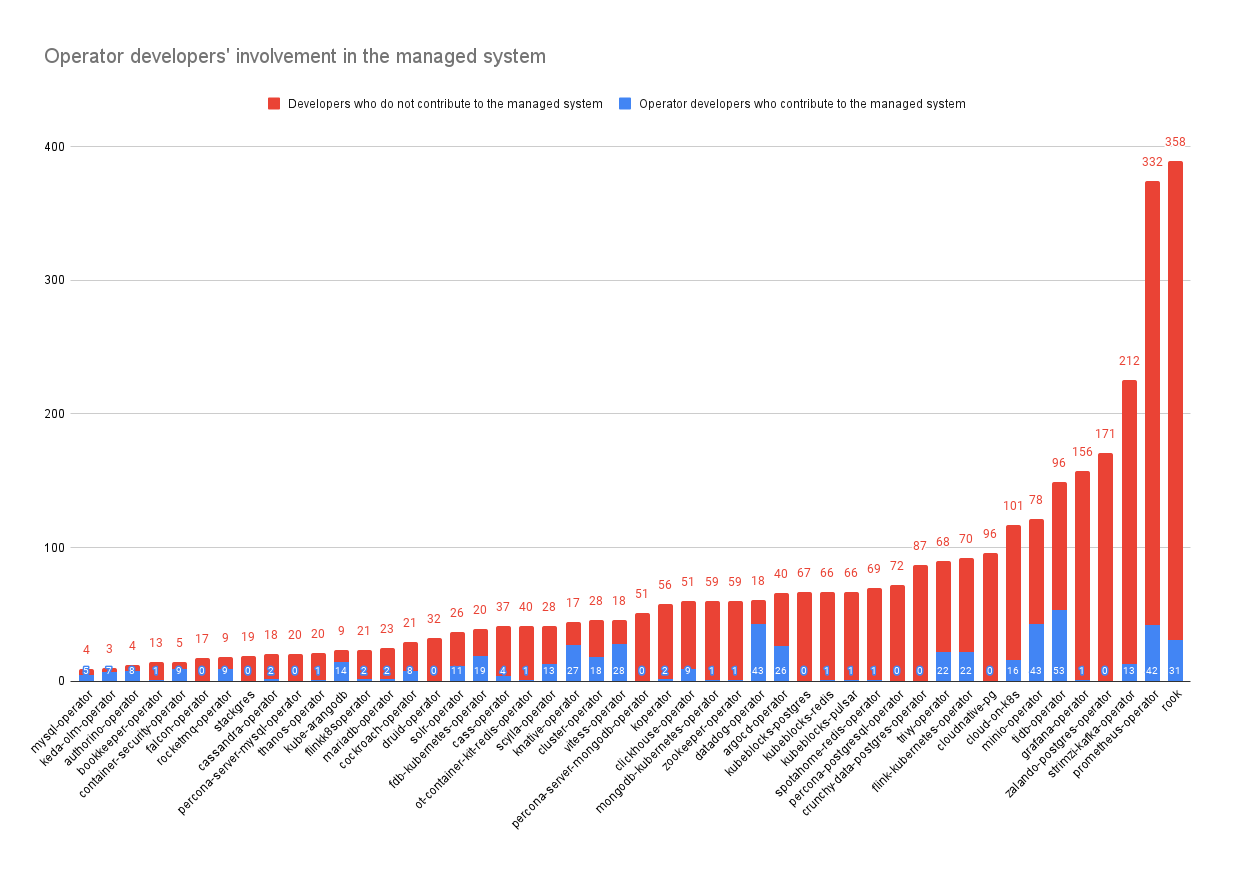
\includegraphics[width=0.95\textwidth,height=9cm]{figures/operator-contributor-involvement-breakdown.png}
    \caption{Operator developers' involvement in the managed system developement}
    \label{fig:contributor}
\end{figure*}

\begin{figure*}
    \centering
    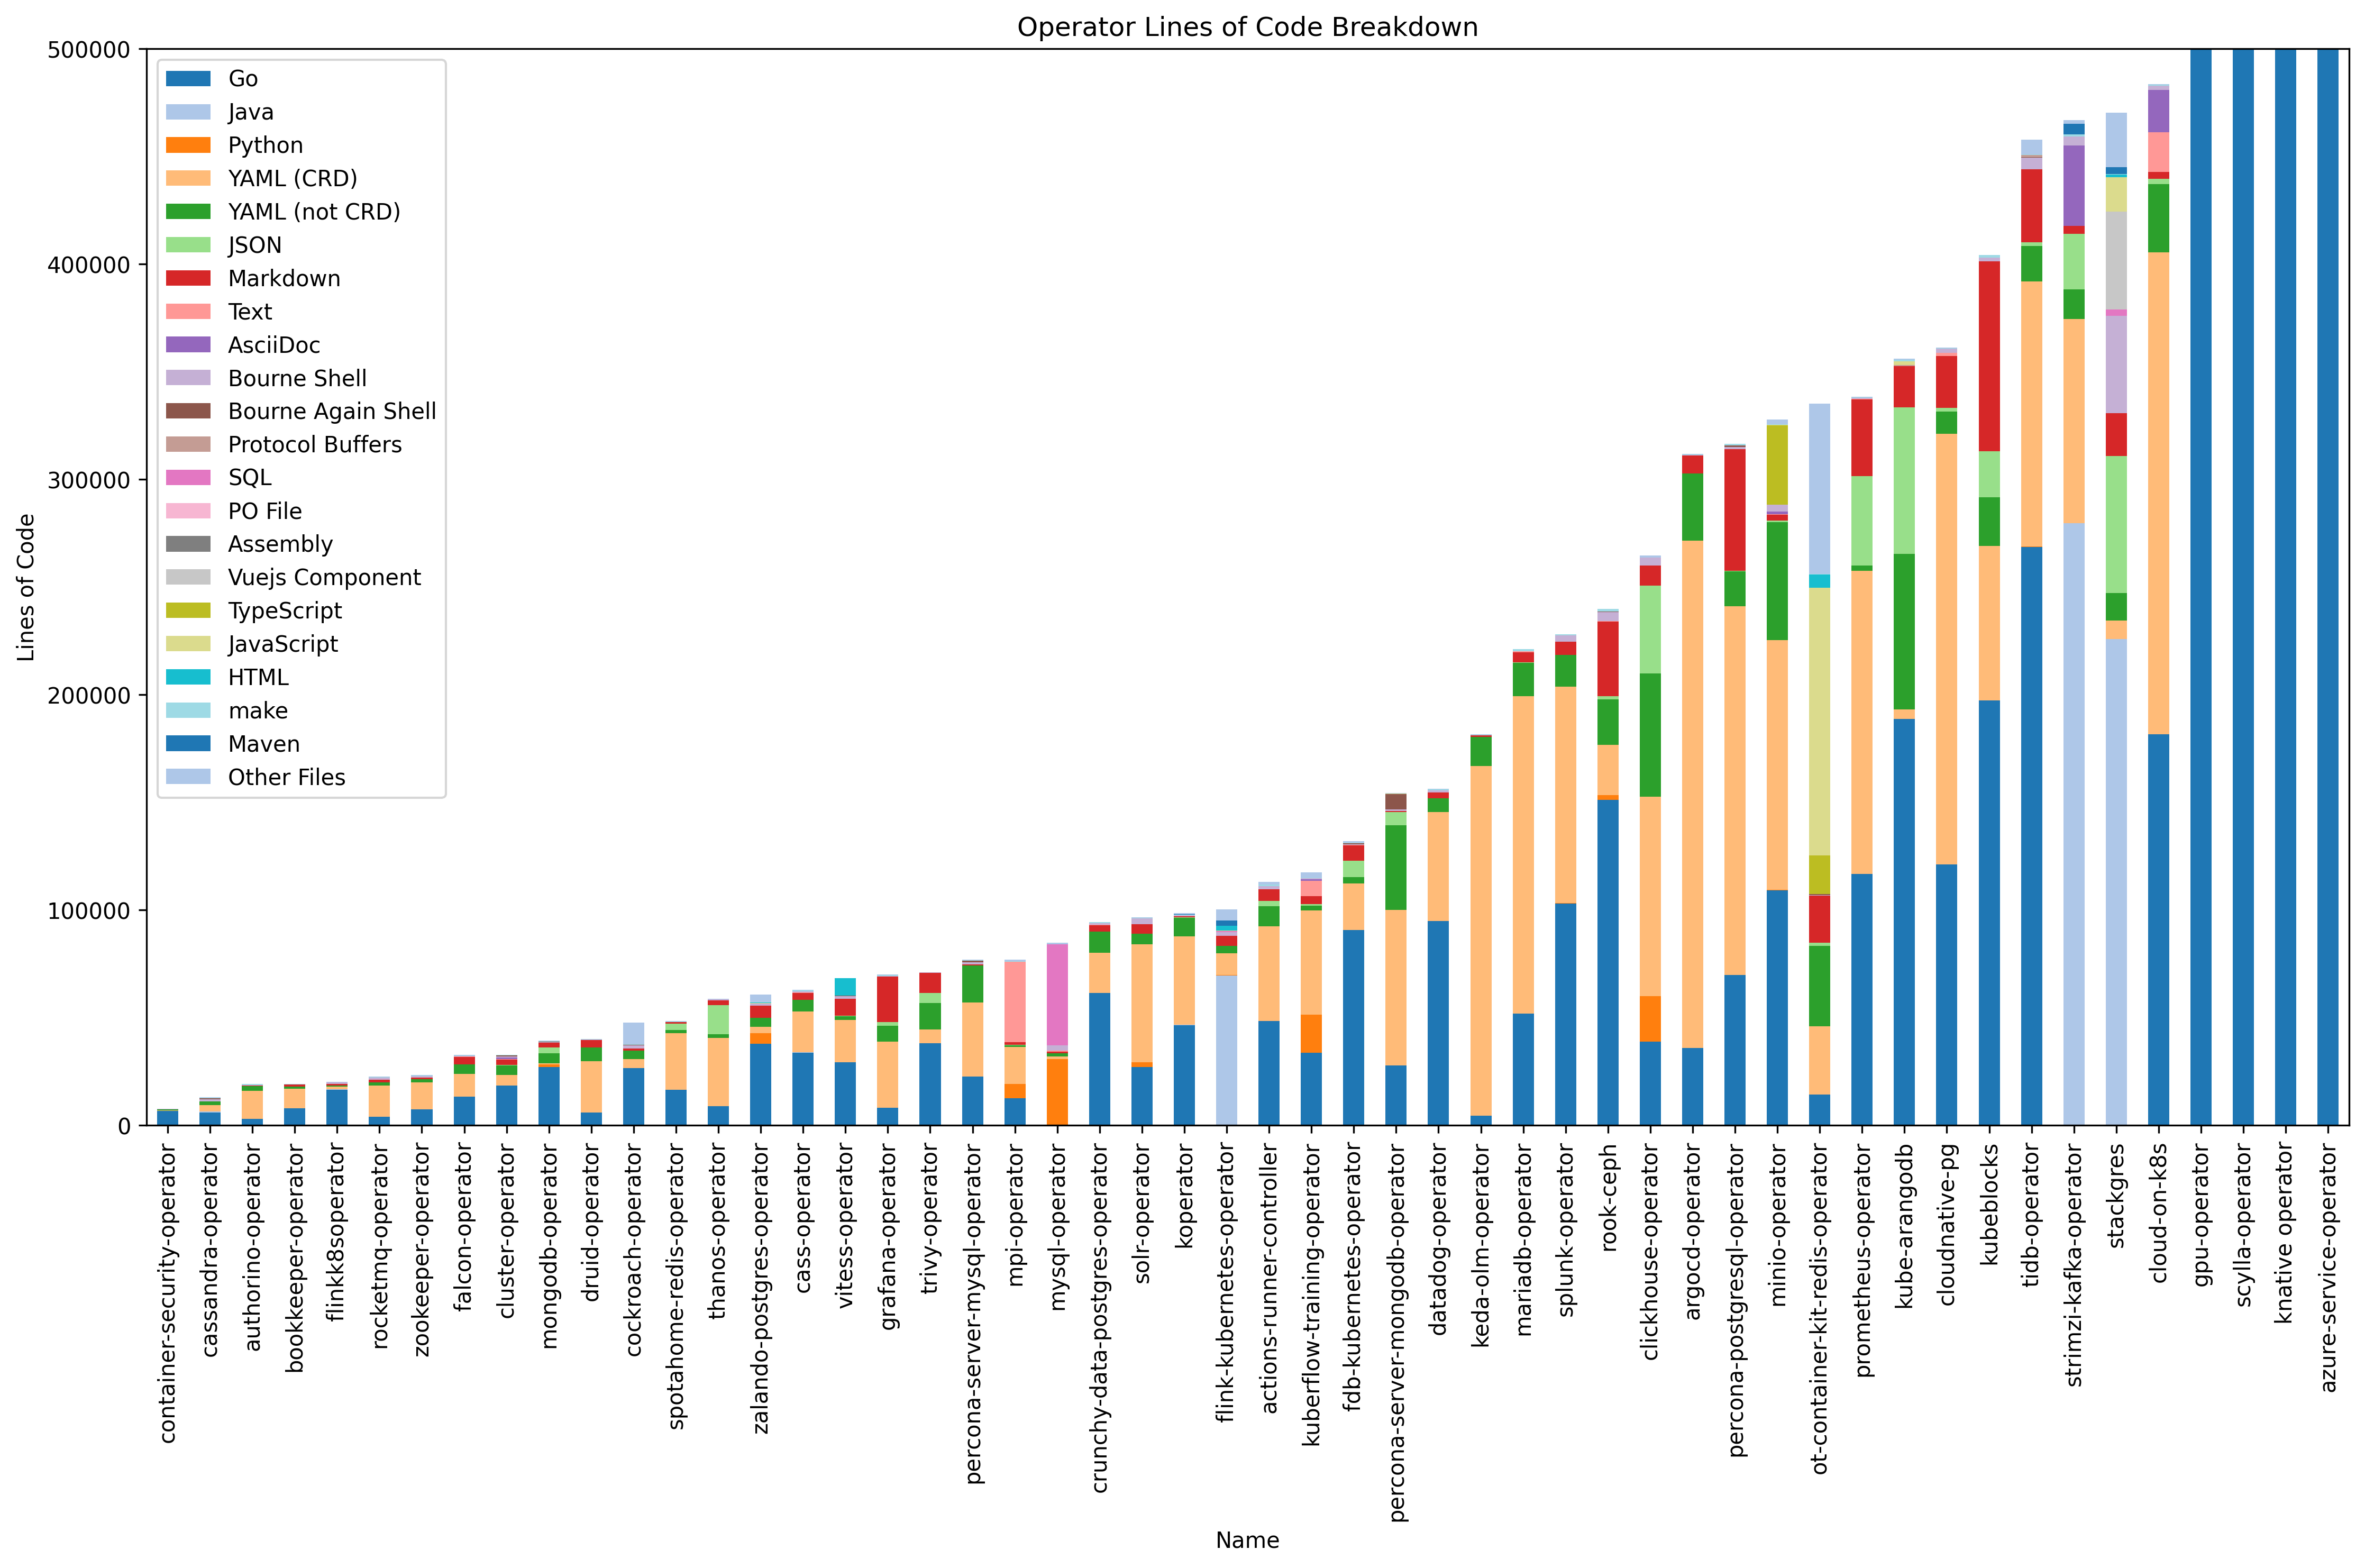
\includegraphics[width=0.95\textwidth,height=9cm]{figures/operator-loc-bar.png}
    \caption{LOC and programming language distribution over operators}
    \label{fig:loc}
\end{figure*}

% \begin{figure}
%     \centering
%     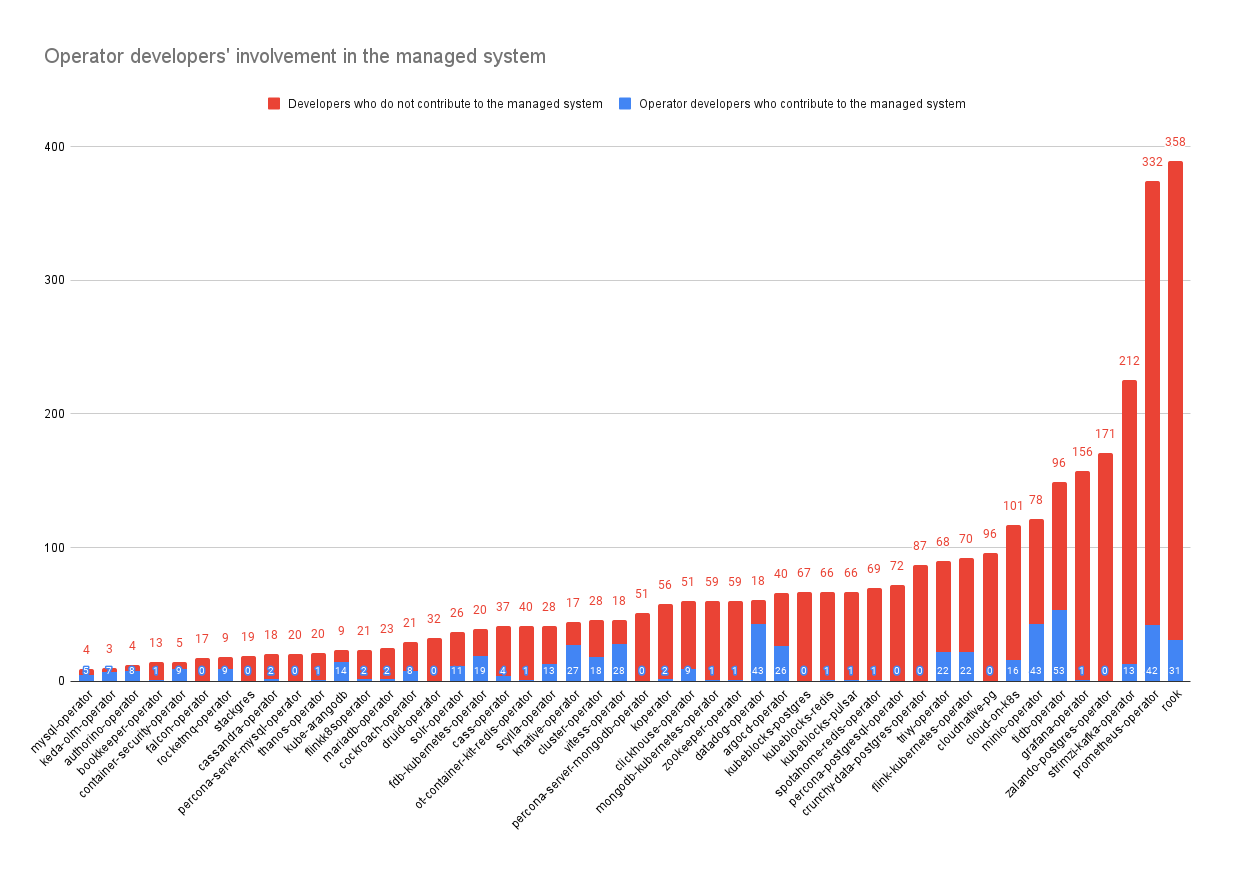
\includegraphics[width=0.95\linewidth]{figures/operator-contributor-involvement-breakdown.png}
%     % \vspace{-18pt}
%     \caption{Popularity of Azure Storage APIs, measured by the number of tests that
%         use an API across all the studied projects.}
%     \label{fig:contributor}
%     \vspace{-15pt}
% \end{figure}

\subsection{What are the developers' challenges?}
Operators are responsible for operating a very specifc managed system and it is
operators' job to reconcile the managed system to the desired state given
users' expectation. Modern software systems can be gigantuous with tens of
thousands lines of code and complicated states management required. This
engenders burdens for operator developers to understand the managed system
thoroughly, increasing the likelyhood for them to make mistakes in developing
the operator.

In \figurename{ \ref{fig:contributor}}, we collect and visualize the
involvement of operator developers in contributing to the managed system using
GitHub repository contributor data. While the absence of operator develoipers'
contribution to the managed system does not necessarily imply their
incompetence in understanding the managed system, it is a still a reflective
metric on the average familiarity of operator developers on the managed system.
In our dataset, only 19\% of the operator projects have more than half of the
developers being contributing to the managed system. The proportion of
developers who are also developing the managed system drops as the operator
project gets larger. In the two largest operator project in our dataset, with
regard to the size of developers, only 10\% of the developers are contributors
to both the managed system and its operator.

\subsection{What are the testing practices of Operators?}
Operators are responsible for managing the state of the managed system. To
ensure the correctness of the operators, developers write tests to verify the
correctness of the operators. We analyze the testing practices of the operators
by counting the number of tests in the operators.

TODO: Add more data and analysis here.

\begin{table}[h]
    \centering
    \begin{tabular}{|c|c|c|}
        \hline
        \textbf{Operator}      & \textbf{Project Stars} & \textbf{Test Cases} \\
        \hline
        Strimzi-Kafka-Operator & 4.3K                   & 1676                \\
        Percona-Xtradb         & 489                    & 130                 \\
        CloudNative-pg         & 3K                     & 1426                \\
        TiDB-Operator          & 1.2K                   & 103                 \\
        MinIO-Operator         & 1.1K                   & 80                  \\
        \hline
    \end{tabular}
    \caption{Automated Test Breakdown by Operator}
    \label{tab:testing}
\end{table}
